\documentclass[a4paper, 12pt, french]{article}
\usepackage[utf8]{inputenc}
\usepackage[T1]{fontenc}
\usepackage{babel}

%Images
\usepackage{graphicx} 
\graphicspath{{src/dev/}}

%Code
\usepackage{listings}
\usepackage{color}

\definecolor{dkgreen}{rgb}{0,0.6,0}
\definecolor{gray}{rgb}{0.5,0.5,0.5}
\definecolor{mauve}{rgb}{0.58,0,0.82}

\lstset{frame=tb,
  language=C,
  aboveskip=5mm,
  belowskip=5mm,
  framesep=3mm,
  showstringspaces=false,
  columns=flexible,
  basicstyle={\small\ttfamily},
  numbers=none,
  numberstyle=\tiny\color{gray},
  keywordstyle=\color{blue},
  commentstyle=\color{dkgreen},
  stringstyle=\color{mauve},
  breaklines=true,
  breakatwhitespace=true,
  tabsize=3
}

%Commandes perso
\newcommand{\hr}{\noindent\rule{13.7cm}{0.4pt}}

%Metas
\title{Réseau}
\author{Elanis - https://github.com/Elanis/LaTeX-cheatsheets}
\date{}

\begin{document}
	\maketitle

	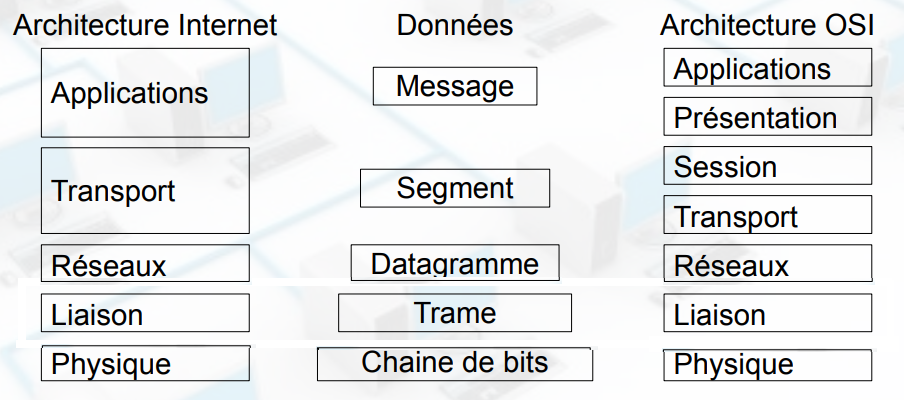
\includegraphics[width=13.8cm]{reseau_modele_osi}

	\section{Introduction}

	« Un réseau est un ensemble d'équipement reliés entre eux et qui échangent des informations »

	\subsection{Echanges sur de longues distances}
	\begin{itemize}
		\item Satellite
		\item Hertzien (TV)
		\item Cable aerien
		\item Antenne Parabolique
		\item Paire torsadée (ADSL, Telephone, etc)
		\item WiMax, Telephonique (2G, 3G, 4G), etc
		\item ...
	\end{itemize}

	\subsection{Echanges sur de courtes/moyennes distances}
	\begin{itemize}
		\item CPL (Courant porteur de ligne): Passage du signal par le réseau éléctrique
		\item NFC (Sans contact): Telephones, Cartes bancaires, Badges, etc
		\item Radio: Bluetooth, WiFi, etc
		\item Femtocell: mini-relai telephonique
		\item Ethernet (de 10 Mbps à 10 Gbps)
		\item ...
	\end{itemize}
	
	\subsection{Internet Mobile}  
	\begin{description}
		\item[2G] GSM/GPRS/EDGE - 384Kbps $\downarrow$ - 188.4Kbps $\uparrow$ - 900-1800 Mhz
		\item[3G] UMTS/3G+ (HSPA+) - 14.4Mbps $\downarrow$ - 5.7Mbps $\uparrow$ - 1900-2100 Mhz
		\item[4G] 4G (LTE) - 100Mbps $\downarrow$ - 50Mbps $\uparrow$ - 800 - 1800 - 2600 Mhz
	\end{description}

	\subsection{Internet Fixe}  
	\begin{description}
		\item[ADSL] 13.7Mbps $\downarrow$
		\item[ADSL 2] 25Mbps $\downarrow$
		\item[VDSL 2] 120Mbps $\downarrow$
		\item[Fibre optique] 200Mbps $\downarrow$
		\item[Internet par satellite] 20Mbps $\downarrow$ - \emph{Note:} Utilisée principalement dans les zones non reliables par les solutions précédentes.
	\end{description}

	\subsection{Le Cloud}

	Le but du cloud est de "dématerialiser" les systèmes informatiques en les envoyant sur le Web. Il en résulte des problèmes sur le réseau avec tout ce nouveau traffic qui auparavant était local aux réseaux d'entreprise le plus souvent. Il exite néanmoins des solutions:

	\subsubsection{Le Edge Computing}

	L'edge computing est une méthode d'optimisation employée dans le cloud computing qui consiste à traiter les données à la périphérie du réseau, près de la source des données. Il est ainsi possible de minimiser les besoins en bande passante entre les capteurs et les centres de traitement des données en entreprenant les analyses au plus près des sources de données.

	\subsubsection{Le Fog Computing}

	Le fog computing consiste à exploiter des applications et des infrastructures de traitement et de stockage de proximité, servant d'intermédiaire entre des objets connectés et une architecture cloud classique.

	\subsection{Niveaux de service}

	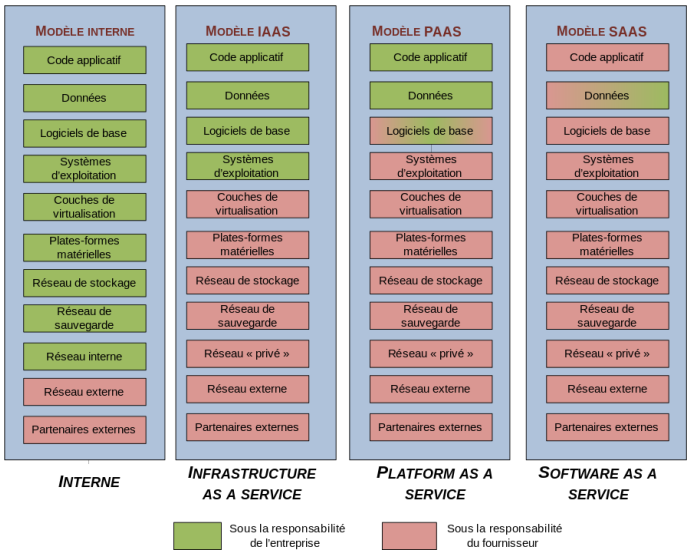
\includegraphics[width=13.8cm]{reseau_niveaux_de_service}

	\section{Physique}

	\emph{Bande passante:} Taille de la bande de frequence utilisée pour transmettre des données

	\emph{Attenuation: } Diminution du signal sur la distance

	\subsection{Supports de transmissions}

	\emph{Particularités diverses: } Bande passante, attenuation, sensibilité, coût, facillité d'installation, etc

	\begin{description}
		\item[Paire torsadée:] dans un même câble par 2, 4 ou 8 fils; une paire est un lien de communication. Chaque paire est enroulée pour limiter les interferences. \emph{Debit Max: 100 Gbps}. Simple, economique, reutilisable, mais sensible aux pertubations électromagnetiques et grande atténuation.
		\item[Coaxial:] il consiste en deux conducteurs ayant le même axe. \emph{Debit Max: 2 Gbps} Tres bonne qualité, haut debit, bonne manipulation mais très cher.
		\item[Fibre optique:] Cylindre de fibre de sillicium extremement fin. \emph{Debit Max: plusieurs terabits par seconde} Bande passante immense, debits très importants, insensibles aux interferences et corrosions chimiques, attenuation faible, leger mais fragile, unidirectionnel, transmission point à point, cout élevé des interfaces.
		\item[Ondes radio:] Wifi (56Mbps), Bluetooth (2Mbps), Infrarouge, Hertzien, etc \emph{Portée jusqu'a quelques centaines de mètres}
		\item[Micro ondes:] Transmission terrestre de 50 à 1000km et satellitaire a 36000km (geostationnaire) ou 800 km d'altitude
	\end{description}


	\subsection{Transmission}

	\subsubsection{Caracteristiques d'un signal}

	Chacun se decompose en une somme infinie de sinusoides (decompostion de Fourrier)

	\emph{Note:} Tout ce qui est hors de la bande passante est naturellement filtré.  

	Rapport signal sur bruit(dB) $ = 10 * log_{10} \frac{S}{B}$ où S est la puissance du signal et B celle du bruit.

	\subsubsection{Capacité d'un canal de transmission}

	\emph{Theoreme de Shannon:} Soient W la bande passante d'un canal de transmission et S/B le rapport signal sur bruit. La capacité en bit/s du canal est :

		$$C = W * log_2 \left( 1 + \frac{S}{B} \right)$$

	\subsection{Numerisation, Quantification, Echantillonnage}

	\emph{Analogique:} Signal continu

	\emph{Numerique:} Signal echantilloné (sur le temps), et quantifié (sur les valeurs) afin d'être stockées et transmises par un equipement electronique.

	\subsubsection{Echantillonnage}

	\emph{Theoreme de Shannon:} Prendre comme max 2 fois la frequence max relevée

	\subsubsection{Quantification}

	Utilisation d'echelles logarithmiques

	\subsubsection{Formules}


	\begin{description}
		\item[Debit binaire ($D_b$)] Nombre max d'elements binaires transmis par seconde
			$$D_r = 1/T_b \ bit/s$$
		\item[Rapidité de modulation ($R_s$)] Vitesse à la queles les symboles se succèdent
			$$ R_s = 1/T_s  \ bauds$$
		\item[Valence (V)] Cardinal de l'alphabet des symboles
			$$ D = R_s * r = R_s * log_2 * V $$
		\item[Debit binaire max] Donne le debit binaire maximum en fonction de la bande passande du canal
			$$ D_{max} = 2 * W * log_2 * V $$
			où W est la largeur de la bande passante et V la valence du signal
	\end{description}

	\subsection{Transmission en bande de base}

	On transmet en bande de base, quand on transmet directement l'information codée sous forme d'un signal carré.

	\begin{description}
		\item[Tout ou rien] 0 est 0 Volt, 1 est +x Volts
		\item[Bipolaire] 0 est 0 Volts, 1 est alternativement +x ou -x Volts. \emph{Permet de mieux distinguer les suites de 1}
		\item[NRZ (No return to zero)] 0 est -x Volts, 1 est +x Volts. \emph{Permet de differencier le silence des 0}
		\item[NRZI (NRZ Inverted space)] 0 est un changement de niveau (entre +x et -x Volts), 1 correspond à une absence de changement.
		\item[RZ (Return to zero)] 0 est 0 Volts, 1 est un front montant (impulsion au milieu du temps bit)
		\item[Biphasé (ou Manchester)] 0 est un front montant, 1 est un front descendant. \emph{Il est plus facile a distinguer grace a un changement de signe à chaque bit}
		\item[Code manchester différentiel] 0 est un front inversé au cycle précédent, 1 est le même front que le cycle précédent.
		\item[Code Miller] 0 est une absence de changement sur l'intervalle, 1 est un front montant/descendant sur l'intervalle
 	\end{description}

	\subsection{Transmission modulée}

	Le principal problème de la transmission en bande de base est que le signal se degrade sur la distance, il est donc utilisé uniquement sur des réseaux locaux. On utilise donc pour de plus grandes distances des signaux sinuisoidaux générés et recupérés par des modems (modulateur - demodulateur).

	Afin d'y introduire de l'information, les modulations permettent de transformer:
	\begin{itemize}
		\item L'amplitude
		\item La fréquence
		\item La phase
	\end{itemize}

	\subsubsection{Modulation d'amplitude}

	Il s'agit d'associer un symbole à chaque amplitude.

	\emph{Avantages:} Moins couteux et plus précis qu'un signal carré, la modulation d'amplitude est simple.
	
	\emph{Désavantages:} Sensibles aux perturbations électromagnétiques (orage, ligne éléctrique, ...)

	\subsubsection{Modulation de fréquence}

	Il s'agit d'associer un symbole à chaque fréquence.

	\emph{Avantages:} Moins couteux et plus précis qu'un signal carré, résistant aux pertubations (d'amplitude).
	
	\emph{Désavantages:} Système de démodulation moins simple à concevoir

	\subsubsection{Modulation de phase}

	Il s'agit d'associer un symbole à des changements de phases.

	\emph{Avantages:} Les dispositifs de (dé)modulation de phase permettent de coder facilement deux états, résistant aux pertubations (d'amplitude).
	
	\emph{Désavantages:} Système de démodulation pas simple à concevoir

	\subsubsection{Combinaison de modulations}

	Les transmissions modulées peuvent combiner plusieurs formes de modulations simultanées. On représente ces modulations par un diagramme spatial:

	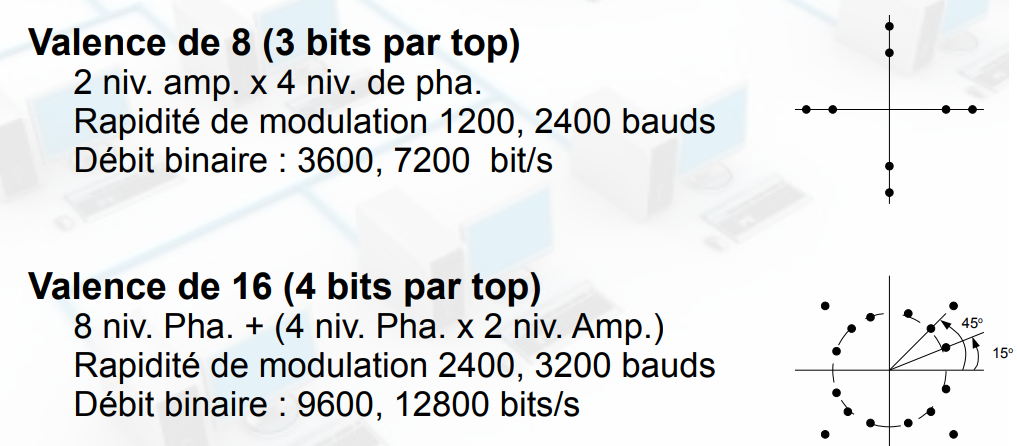
\includegraphics[width=13.8cm]{reseau_diagramme_spatial}

	\section{Liaison}

	Le but de la couche liaison est de transporter les trames d'un nœud à un autre de manère fiable.\\

	\emph{DCE: } Detection et correction d'erreur

	La couche liaison offre 2 fonctions:
	\begin{itemize}
		\item Detection et correction d'erreurs
		\begin{itemize}
			\item Bits de parités
			\item Code Cyclique
		\end{itemize}
		\item Protocoles d'accès au canal
		\begin{itemize}
			\item Protocoles à partitionnement du canal
			\item Protocoles aléatoires
			\item Protocoles à partage de ressources
		\end{itemize}
	\end{itemize}

	Les services de la couche liaison sont:
	\begin{description}
		\item[Encapsulation] incorporer les données de la couche supérieur (réseau) dans une trame
		\item[Accès au médium] protocole d'accès au canal de communication
		\item[Détection / Correction d'erreurs] mécanismes de détection / correction d'erreurs de transmission
		\item[Transmission fiable] service d'acquittement et de retransmission pour certains liens peu fiables (ex. sans fil)
		\item[Contrôle de flux] éviter les surcharges si trop de trames arrivent trop vite sur un nœud
	\end{description}

	Cette couche est souvent impantée sur la carte réseau et est autonome.

	\subsection{Detection et correction d'erreur}

	\subsubsection{Bits de parités}

	Ajouter aux données un bit DCE afin de fixer la parité de la trame (Fixer le nombre de 1 dans la trame: pair ou impair).

	\emph{Limitations:} Le nombre d'erreurs detectable est au maximum de 1, en effet, s'il y'a 2 erreurs, la parité s'annule.

	\subsubsection{Bits de parités bidimensionneles}

	Le principe est le même que le précédent, sauf que les bits de parités sont insérés en ligne et en colonne.

	\emph{Limitations:} Permet de detecter et corriger une erreur, de detecter 2 erreurs sans pouvoir forcement les corriger.

	\emph{Note:} Ce même principe est utilisé dans les lecteurs CD audio

	\subsubsection{Codes cycliques CRC}

	\emph{Principe:}
	\begin{itemize}
		\item On désire envoyer une trame \emph{D} de \emph{d} bits, à laquelle on ajout un DCE \emph{R} de \emph{r} bits
		\item Les deux cotés se mettend d'accord sur une suite de \emph{r+1} buts qu'on appellera \emph{G} pour générateur
		\item L'émetteur envoie le message qui contient \emph{(D, R) (d + r bits)} de telle sorte que le message soit divisible par \emph{G}.
	\end{itemize}

	\emph{Verification:} Le récepteur recoit le message, le divise par \emph{G}, et si il reste 0 il n'y a pas d'erreur.\\

	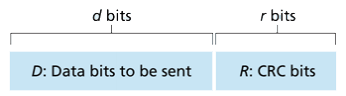
\includegraphics[width=8cm]{reseau_crc_principe}

	\emph{Remarques:}
	\begin{itemize}
		\item En ajoutant \emph{R} à \emph{D}, on crée un message divisible par \emph{G}, c'est pour cela que \emph{R} est le reste de la division.
		\item Les CRC sont normalisés selon la taille de leur générateur. Exemple: CRC-32 a un générateur de 32 bits
		\item Chaque CRC peut detecter des erreurs de largeur \emph{r} bits ou moins.
	\end{itemize}

	\subsection{Protocoles d'accès au canal}

	Il existe deux types de liens: point à point (deux nœuds se partagent un canal), ou diffusion (canal partagé par plusieurs nœuds). Sur un canal partagé, les nœuds qui transmettent des trames en même temps, ce qui peut engender des \emph{collisions}. Ces collisions brouillent les trames les rendant illisibles.

	\subsubsection{Protocoles à partionnement du canal}

	Il s'agit de diviser la bande passante et/ou le temps de parole equitablement pour chaque nœud.

	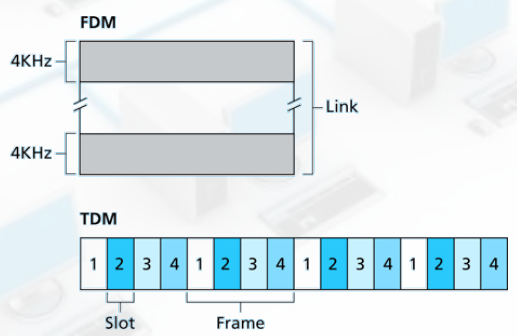
\includegraphics[width=13.8cm]{reseau_partitionnement_canal}

	\subsubsection{Protocoles à accès aléatoires}

	Tout les nœuds profitent de tout le débit et transmettent quand ils le desirent. S'il detectent une collision, il retransmettent après un temps aléatoire. Le processus est réitéré jusqu'a ce que la trame soit transmise.

	\subsubsection{Protocoles ALOHA à allocation temporelle}

	Le temps est divisé en intervalles egaux pour tous, où transmettre une trame. Les nœuds sont synchronisés temporellement.

	\emph{Deroulement:}
	\begin{itemize}
		\item Attendre le début du prochain intervalle pour transmettre une trame
		\item Si pas de collisions, on passe à la trame suivante (puis revenir au début)
		\item Si il y a eu collision
		\begin{itemize}
			\item avec probabilité p on retransmet la trame (puis revenir au début)
			\item avec probabilité (1-p) on laisse passer l'intervalle (puis revenir au début)
		\end{itemize}
	\end{itemize}

	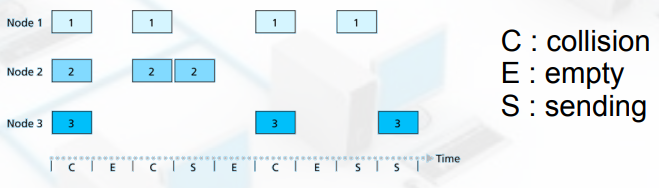
\includegraphics[width=13.8cm]{reseau_aloha}

	\subsubsection{Protocoles ALOHA pur}

	Il n'y a plus de synchronisation du temps, le nœud transmet la trame dès qu'il la recoit des couches supérieures.

	\emph{Deroulement:}
	\begin{itemize}
		\item S'il n'y a pas de collision, on passe à la trame suivante
		\item Si il y a eu collision
		\begin{itemize}
			\item avec probabilité p on retransmet la trame
			\item avec probabilité (1-p) attendre un moment (le temps nécessaire pour transmettre une trame)
			\item revenir à 1
		\end{itemize}
	\end{itemize}

	\subsubsection{Protocole CSMA/CD - Carrier Sense Multiple Access with Collision Detection}

	\emph{Deroulement:}
	\begin{itemize}
		\item On écoute le canal
		\begin{itemize}
			\item si il n'y a pas de trame qui transite, on envoie la trame
			\item si il y a une trame, on attend un temps aléatoire avant d'écouter à nouveau
		\end{itemize}
	\end{itemize}
	Si une fois qu'on a commencé à émettre, on détecte une collision, on arrête de transmettre et on attend un temps aléatoire.

	\subsubsection{Protocoles à partage de ressources}

	\emph{Deux propriétés désirables pour un protocole d'accès:}
	\begin{itemize}
		\item si un seul nœud actif, lui donner tout le débit (\emph{R} bits/s)
		\item si \emph{M} nœuds actifs, leur assurer un débit moyen de \emph{R/M} bits/s
	\end{itemize}

	ALOHA ET CSMA possèdent la première propriété mais pas la secondent. De plus, les latences de temps introduisent des intervalles ou rien ne transite, et donc une perte de débit.

	\subsubsection{Protocole à sondages}

	Un nœud maitre sont les autres nœuds à tour de rôle afin de leur indiquer qu'il peuvent transmettre.
	\emph{Deroulement:}
	\begin{itemize}
		\item le maître sonde le \emph{i} ème nœud et lui indique qu'il peut transmettre jusqu'à \emph{p} trames
		\item Si le nœud a des trames à transmettre, il le fait, pendant que le nœud maître attende
		\item Une fois terminé, le maître passe au \emph{i+1} ème nœud
	\end{itemize}

	\emph{Avantages:} Pas de collisions, pas de temps d'inactivité dans le reseau
	\emph{Désavantages:} Un delai de sondage (s'il n'y a qu'un seul nœud actif, le nœud maitre les sondes quand même tous) et si le maitre tombe en panne, il n'y a plus de transmissions.

	\subsubsection{Protocole à passage de jetons}

	Un nœud attend d'avoir le jeton pour transmettre. Le jeton est un signal (chaîne de bits) particulier qui passe entre les nœuds.

	\emph{Deroulement:}
	\begin{itemize}
		\item Un nœud prend le jeton du canal
		\item s'il a des trames à transmettre
		\begin{itemize}
			\item il peut en envoyer un nombre maximum
			\item il remet le jeton sur le canal et le transmet au nœud voisin
			\item s'il lui reste des trames, il attend le prochain passage du jeton
		\end{itemize}
		\item sinon il envoie directement le jeton à son voisin
	\end{itemize}

	\emph{Avantages:} Très efficace
	\emph{Désavantages:} Si un nœud tombe en panne, le jeton ne transite plus. Si un nœud "oublie" de remettre le jeton sur le lien, la transmissions s'arrête. Un nouveau jeton doit être régénéré.

\end{document}